\documentclass[../../main/main.tex]{subfiles}
\begin{document}
\section{Nash Equilibrium Strategy Profile}

Having established the equilibrium structure in Section \ref{sec:solving_lcp} and derived the indifference equations in Section \ref{subsec:constraints}, we now present the complete solution. The system of equations from Section \ref{subsec:constraints} was solved symbolically using Mathematica (see Appendix \ref{app:ma} for the complete code), yielding closed-form expressions for all threshold values and strategic functions.

\begin{theorem}[LCP Nash Equilibrium]
    \label{thm:nash_equilibrium}
LCP has a unique Nash equilibrium strategy profile in which the bettor's strategy is monotone-admissible (up to measure zero sets of hands for each player). This strategy profile is given by:

\begin{align*}
    x_{0} &= \frac{3 t^{2} \left(t - 1\right)}{r^{3} + t^{3} - 7}\\
    x_{1} &= \frac{- 2 r^{3} + 3 r^{2} + t^{3} - 1}{r^{3} + t^{3} - 7}\\
    x_{2} &= \frac{r^{3} + t^{3} - 1}{r^{3} + t^{3} - 7}\\
    x_{3} &= \frac{r^{3} - 3 r + t^{3} - 4}{r^{3} + t^{3} - 7}\\
    x_{4} &= \frac{r^{3} + 3 r^{2} - 6 r + t^{3} - 4}{r^{3} + t^{3} - 7}\\
    x_{5} &= \frac{r^{3} + t^{3} + 3 t^{2} - 7}{r^{3} + t^{3} - 7}\\
    b_{0} &= \frac{t^{3}}{r^{3} + t^{3} - 7}\\
    b(s) &= \frac{t^{3} \left(s+1\right)^3 - (3s + 1)}{\left(r^{3} + t^{3} - 7\right) \left(s+1\right)^3}\\
    c(s) &= \frac{r^{3} + t^3 -1 + s \left(r^{3} + t^{3} - 7\right)}{\left(s + 1\right) \left(r^{3} + t^{3} - 7\right)}\\
    v(s) &= \frac{r^{3} + t^{3} -1 + \left(r^{3} + t^{3} - 7\right) \left(2 s^{2} + 4 s + 1\right)}{2 \left(r^{3} + t^{3} - 7\right) \left(s^{2} + 2 s + 1\right)}
\end{align*}

where $r = L/(1+L)$ and $t = 1/(1+U)$.

\noindent\textbf{Remark:} The change of variables to $(r, t)$ significantly simplifies the expressions compared to the original $(L, U)$ formulation. This transformation reveals underlying symmetries and makes many properties more transparent, as we will see in the analysis of game value and parameter effects.

% \begin{align*}
%     x_0 &= \frac{3 (L+1)^3 U}{A_4}\\
%     x_1 &= \frac{3 A_0 L U+A_0 U-L^3-3 L^2}{A_4}\\
%     x_2 &= \frac{A_5}{A_4}\\
%     x_3 &= \frac{A_2 L^3+3 A_2 L^2+3 L \left(5 U^3+15 U^2+15 U+4\right)+4 U^3+12 U^2+12 U+3}{A_4}\\
%     x_4 &= \frac{3 A_1 L^2+A_2 L^3+3 A_2 L+4 U^3+12 U^2+12 U+3}{A_4}\\
%     x_5 &= \frac{3 A_3 L^2+3 A_3 L+A_3+L^3 \left(6 U^3+18 U^2+15 U+2\right)}{A_4}\\
%     b_0 &= -\frac{(L+1)^3}{\text{A4}} \\ 
%     b(s) &= b_0 - \frac{(1+3s)(x_2-1)}{6(1+s)^3}\\
%     c(s) &= \frac{x_2+s}{s+1}\\
%     v(s) &= \frac{x_2+2 s^2+4 s+1}{2 (s+1)^2},
% \end{align*}

% where the common subexpressions are:

% \begin{align*}
% 	A_0 &= U^2+3 U+3 \\
%     A_1 &= 7 U^3+21 U^2+21 U+6 \\
%     A_2 &= 6 U^3+18 U^2+18 U+5 \\
%     A_3 &= 7 U^3+21 U^2+18 U+3 \\
%     A_4 &= 3 A_1 L^2+3 A_1 L+A_1+A_2 L^3 \\
%     A_5 &= 3 A_0 L^2 U+3 A_0 L U+A_0 U-L^3.
% \end{align*}
\end{theorem}

Refer back to Section \ref{subsec:nash_equilibrium_structure} for an explanation of how these values fit together to actually form the strategy profile.

A proof of this theorem can be found in Appendix \ref{app:nash_equilibrium}.

This solution is more interpretable in graphical form. Figure \ref{fig:strategyprofile} shows the strategy profile for various values of $L$ and $U$ ranging from very lenient ($L=0, U=10$) to very restricted ($L=0.5, U=1$). The more lenient bet size limits model something closer to NLCP, while the more restricted bet size limits model something closer to FBCP with a fixed bet size. Indeed, we see that the strategy profile for $L=0, U=10$ looks qualitatively similar to the strategy profile of NLCP---we will show in Section \ref{sec:strategic_convergence} that the strategy profile approaches the Nash equilibrium of NLCP as $L$ and $U$ approach $0$ and $\infty$, respectively, and that the strategy profile approaches the Nash equilibrium of FBCP as $L$ and $U$ approach some fixed value $s$ from either side.

\begin{figure}[h!]
    \begin{adjustwidth}{-1in}{-1in}
        \centering
        \begin{minipage}{0.6\textwidth}
            \centering
            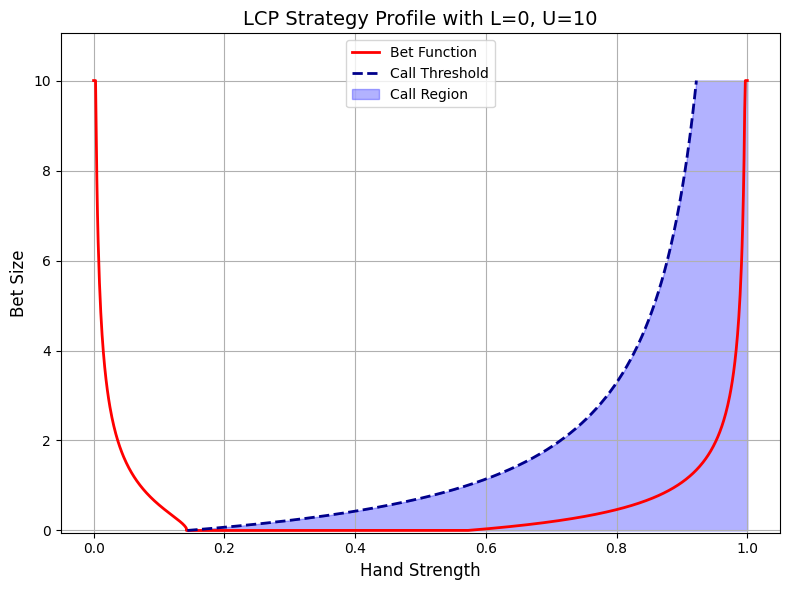
\includegraphics[width=\textwidth]{images/LCP_profile_0_10.png}
        \end{minipage}
        \hspace{0.05\textwidth}
        \begin{minipage}{0.6\textwidth}
            \centering
            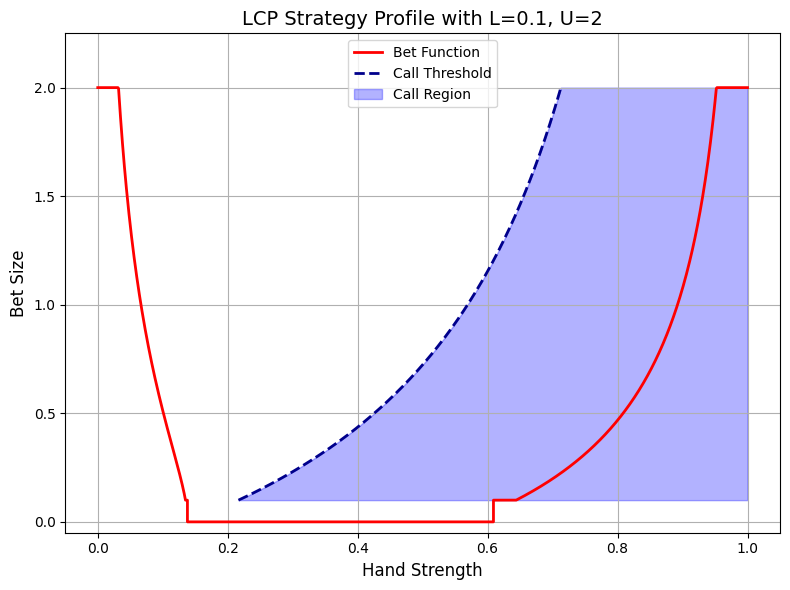
\includegraphics[width=\textwidth]{images/LCP_profile_0.1_2.png}
        \end{minipage}
        \vspace{0.5cm}\\
        \begin{minipage}{0.6\textwidth}
            \centering
            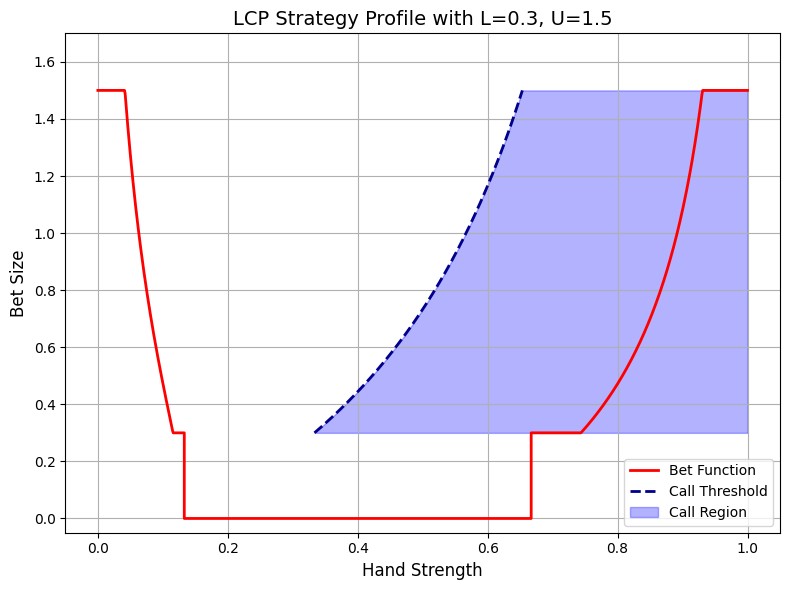
\includegraphics[width=\textwidth]{images/LCP_profile_0.3_1.5.png}
        \end{minipage}
        \hspace{0.05\textwidth}
        \begin{minipage}{0.6\textwidth}
            \centering
            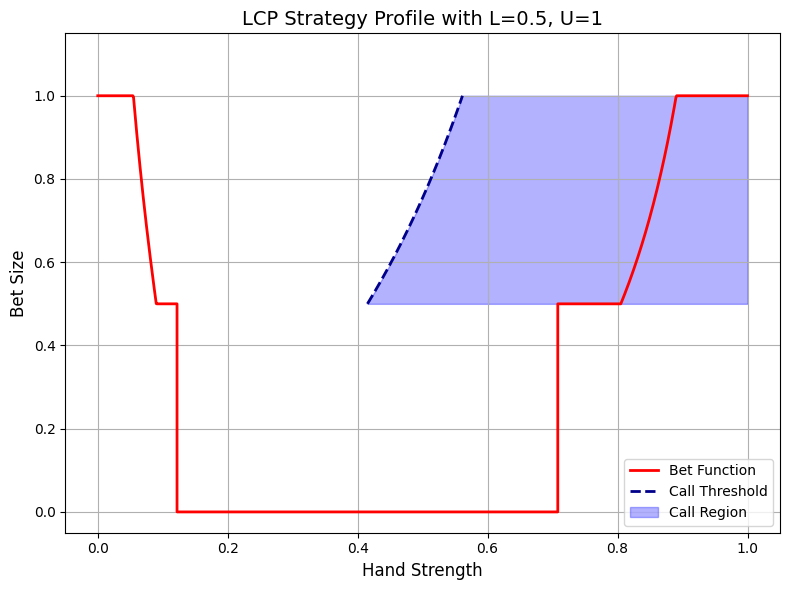
\includegraphics[width=\textwidth]{images/LCP_profile_0.5_1.png}
        \end{minipage}
    \end{adjustwidth}
    \caption{Nash equilibrium strategy profiles for different values of $L$ and $U$, from very lenient to very restricted bet sizes. The bet function maps hand strengths to bet sizes, while the call function gives the minimum calling hand strength for a given bet size. The shaded regions represent the hand strengths for which the caller should call a given bet size.}
    \label{fig:strategyprofile}
\end{figure}


\end{document}
